\setlength{\headheight}{13.59999pt}

This chapter is concerned with the method that we have used to create semi-analytic models of planet wakes.
These models encompass both the linear and non-linear disk response caused by a perturbing planet as described in the previous chapter. 
This work builds on that presented in \citet{bollati2021} and so we will be predominantly concerned with the differences between our methods.
However we aim to provide enough detail to be understandable without having read the aforementioned paper.
The chapter concludes with an application of the analytics\footnote{We will use the terms analytic and semi-analytic interchangeably from now on.}, where we model the kinematic arc detected in the disk of HD~169142 in order to constrain the mass of a potential embedded planet in the disk.

\section{Wakeflow: A Python Package For Semi-Analytic Models of Planet Wakes} \label{sec:JOSS}

This section has been submitted to the Journal of Open Source Science and is currently in review. The preprint is publicly available here: \url{https://github.com/TomHilder/wakeflow/blob/master/paper/paper.md}

\subsubsection{Summary}

\textsc{wakeflow} is a Python package for generating semi-analytic models of the perturbations induced by planets embedded in gaseous circumstellar disks. 
These perturbations take the form of a spiral shock wave \citep{ogilvie2002}, and are often called a ``planet wake'' in analogy with that produced by a boat in a lake.

\subsubsection{Statement of Need}

Detecting newly formed planets embedded in their disk is a challenging problem in the field of planet formation. 
A major area of progress in recent years is the detection of planets by the gravitationally induced disturbance in their host disks. 
This disturbance, caused by the planet wake, manifests as a deviation in velocity from the bulk flow which may be measured through the Doppler shift of molecular lines \citep[e.g.][]{perez2015, pinte2018a}. 
Such kinematic observations have been accurately reproduced through 3D fluid simulations of the planet-disk interaction, allowing for the inference of planet and disk properties \citep{pinte2018a, pinte2019}. 
However, these studies are computationally expensive.

\textsc{wakeflow} eases this computational cost by applying the theory of planet wake generation and propagation \citep{goldreich1979,goodman2001,rafikov2002a,bollati2021} to create semi-analytic models of planet wakes. 
\textsc{wakeflow} models are readily created in a few seconds on a modern laptop, as opposed to the hours of supercomputer time needed for 3D hydrodynamical simulations. 
The relatively low computational cost of \textsc{wakeflow} means that researchers can get an idea of whether planet-disk interactions can explain their observations, and the disk and planet parameters needed, before spending computer time on more detailed simulations.

\textsc{wakeflow} can interface with the radiative transfer code \textsc{mcfost} \citep{pinte2006,pinte2009} in order to create synthetic observations of the semi-analytic models for direct comparison with observed continuum or line emission.

\textsc{wakeflow} is partially adapted from a previous Python code also written by us called \textsc{analytical\_kinks} \citep{bollati2021a}. 
\textsc{wakeflow} is intended to be a more complete, versatile and easy to use version of that code, and it obeys standard Python packaging conventions.
In addition, \textsc{wakeflow} can directly interface with \textsc{mcfost} while \textsc{analytical\_kinks} cannot.
At the time of writing, no other open source software packages exist to generate the perturbations induced by an embedded planet in a circumstellar disk using the semi-analytic theory of planet wakes.

Existing scientific publications focusing on detecting the kinematic signatures of planets that have used \textsc{wakeflow} or its predecessor \textsc{analytical\_kinks} include \citet{bollati2021}, \citet{calcino2022}, \citet{teague2022}, \citet{garg2022} and \citeauthor{fasanoinprep.} (in prep.).

\subsubsection{Acknowledgements}

\textsc{wakeflow} relies on the following scientific Python packages: \textsc{NumPy} \citep{harris2020}, \textsc{matplotlib} \citep{hunter2007}, \textsc{SciPy} \citep{virtanen2020} and \textsc{Astropy} \citep{astropycollaboration2022}.

\section{Semi-Analytic Solution Algorithm}

\begin{figure}
    \centering
    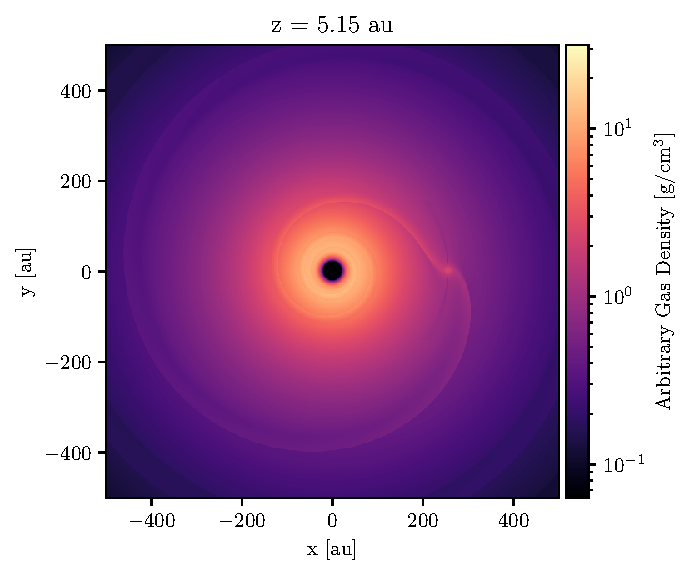
\includegraphics[width = 0.85\textwidth]{figures/wakeflow_tutorial_plot.pdf}
    \caption{Density slice of a \textsc{wakeflow} model at constant height $z=5.15$ au, plotted with a logarithmic colourbar. The model contains a $0.5 \, \mathrm{M_J}$ planet, placed at a separation of $256$ au from the central star. These results were generated following the quickstart tutorial publicly available on the \textsc{wakeflow} documentation\protect\footnotemark, and are meant as a model of the planet wake in the disk of HD~163296, with disk parameters chosen following \citet{pinte2018a} and \citet{calcino2022}.}
    \label{fig:example_model}
\end{figure}

\footnotetext{\url{https://wakeflow.readthedocs.io/en/latest/tutorials/quickstart.html}}

Here we provide an overview of the algorithm used by \textsc{wakeflow} to generate models.
For stages that are sufficiently different to \citet{bollati2021}, further detail will be provided in the section \ref{sec:model_considerations}.
The algorithm proceeds as:
\begin{enumerate}
    \item The global grid geometry is generated based on the user's choice of grid geometry and number of grid points. Both cylindrical and cartesian grid geometries are supported, as well as the \textsc{mcfost} grid geometry if the user wishes to generate synthetic observations from their model.
    
    The run time for \textsc{wakeflow} scales linearly in the number of grid points $n_x \times n_y$ or $n_r \times n_\phi$, but is roughly independent of the number of points in the vertical direction $n_z$..
    
    \item The unperturbed disk density and velocity structure is calculated based on the user's choice of disk parameters as outlined in section \ref{sec:diskstruct}.
    
    \item The linear perturbations are calculated and mapped onto the global disk geometry, following section \ref{sec:linear_box}. The perturbations $\sigma, u$ and $v$ are assumed to be independent of vertical height $z$.
    
    \item The initial conditions for the non-linear evolution are extracted from the edge of the linear regime along a slice of constant $t$, as described in \ref{sec:transformations}.
    
    \item Burger's equation is solved in $(t,\eta)$ space until $t_{\rm f}=300$ using a vectorised Godunov solver \citep{astrofluids}. Unlike in \citet{bollati2021} we use make use of adaptive time-steps, which both ensures the stability of the solution (especially for large planet masses that shock quickly), as well as improves efficiency as large time-steps are taken when appropriate. After $t_{\rm f}$, the asymptotic solution is taken as described in \citet{bollati2021}.
    
    \item The solution $\chi(t,\eta)$ is transformed to $\chi(r,\phi)$ as described in section \ref{sec:transformations}.
    
    \item The density perturbations in the non-linear regime are calculated from $\chi$ using equations \ref{eq:chi} and \ref{eq:g_power}. The velocity perturbations are calculated from $\chi$ as described in section \ref{sec:velocity_perts}. Again, all perturbations $\sigma, u$ and $v$ are assumed to be independent of $z$.
    
    \item The results are written to the disk. This output may be a \textit{.fits} file if desired.
\end{enumerate}

\noindent A density slice of an example \textsc{wakeflow} model is shown in Figure \ref{fig:example_model}.
This model was calculated on a $1000 \times 1000 \times 30$ grid in $x,y$ and $z$ respectively, and took in $19.1$ seconds to compute on an Apple M1 processor.

\section{Theoretical and Numerical Considerations} \label{sec:model_considerations}

\subsection{Unperturbed Disk Structure} \label{sec:diskstruct}

Here we outline the unperturbed disk model used in \textsc{wakeflow} onto which the perturbations are added.

\subsubsection{Temperature}

We assume that the sound speed $c$ obeys a simple radial power law 
\begin{align}
    c \propto r^{-q},
\end{align}
where $q$ is some real number. Thus the disk temperature scales as 
\begin{align}
    T \propto c^2 \propto r^{-2q}.
\end{align}
The constant of proportionality for these relations in determined by the user specified value of the disk aspect ratio $H/r$ at $r=r_{\rm ref}$

\subsubsection{Density}

We use a density structure derived by assuming that the disk is in vertical hydrostatic equilibrium \citep{pringle1981}, but unlike in \ref{eq:vertical_rho} we will not assume that $z\ll r$.
The density $\rho$ is given by 
\begin{align}
    \rho(r,z) \propto \left( \frac{r}{r_{\rm ref}} \right)^{-p} \exp{\left( \frac{G M_\star}{c^2} \left[ \frac{1}{\sqrt{r^2 + z^2}} - \frac{1}{r} \right] \right)},
\end{align}
where $p$ is some real number. 
The constant of proportionality is set directly by the user, or calculated by \textsc{mcfost} based on the total gas mass.

Very commonly the density profile is parameterised in terms of the surface density $\Sigma$, not the actual density $\rho$ as above.
If the surface density is parameterised as $\Sigma \propto r^{-\delta}$ where $\delta$ is some real number, then equation \ref{eq:surf_dens_to_dens} gives the approximate relation 
\begin{align}
    p \simeq \frac{3}{2} - q + \delta,
\end{align}
which can be used to convert between density parameterisations.
This conversion is only approximate in our context, since is does assume that $z \ll r$ and our density profile does not.
However this turns out not to matter since $\delta$ will only show up in the $t(r)$ mapping which we will assume is the same for all $z$.

\subsubsection{Velocities}

The radial and vertical motions in the unperturbed disk are set to zero. 
The rotation is derived assuming radial force balance \citep[e.g.][]{nelson2013} and is given by 
\begin{align}
    \Omega(r,z) = \Omega_{\rm K} \left[ - \left(p + 2q\right) \left( \frac{H}{r} \right)^2 + \left( 1-2q \right) + \frac{2qr}{\sqrt{r^2 + z^2}}\right]^{1/2}, \label{eq:omega_wf_ps}
\end{align}
where $\Omega_{\rm K}$ is as defined in equation \ref{eq:point_pot}.

\subsection{Linear Box} \label{sec:linear_box}

The solution in the linear regime nearby the planet used in \textsc{wakeflow} was calculated by \citet{bollati2020} and \citet{bollati2021} by solving equations \ref{eq:fourier_v} -- \ref{eq:fourier_sigma} numerically following the procedure outlined in \citet{goodman2001}.
Here, we simply read their dimensionless calculations and scale them accordingly for our purposes. Figure \ref{fig:lin_box_bollati} shows the $u$ and $v$ solutions presented in \citet{bollati2021} in local cartesian coordinates $x,y$ centred on the planet location.
The $x,y$ coordinates are scaled by the Mach-1 length $l_{\rm p} = 2H_{\rm p}/3$, while the perturbation are scaled by the planet mass in units of the thermal mass $M_{\rm p} / M_{\rm th}$.

\begin{figure}
    \centering
    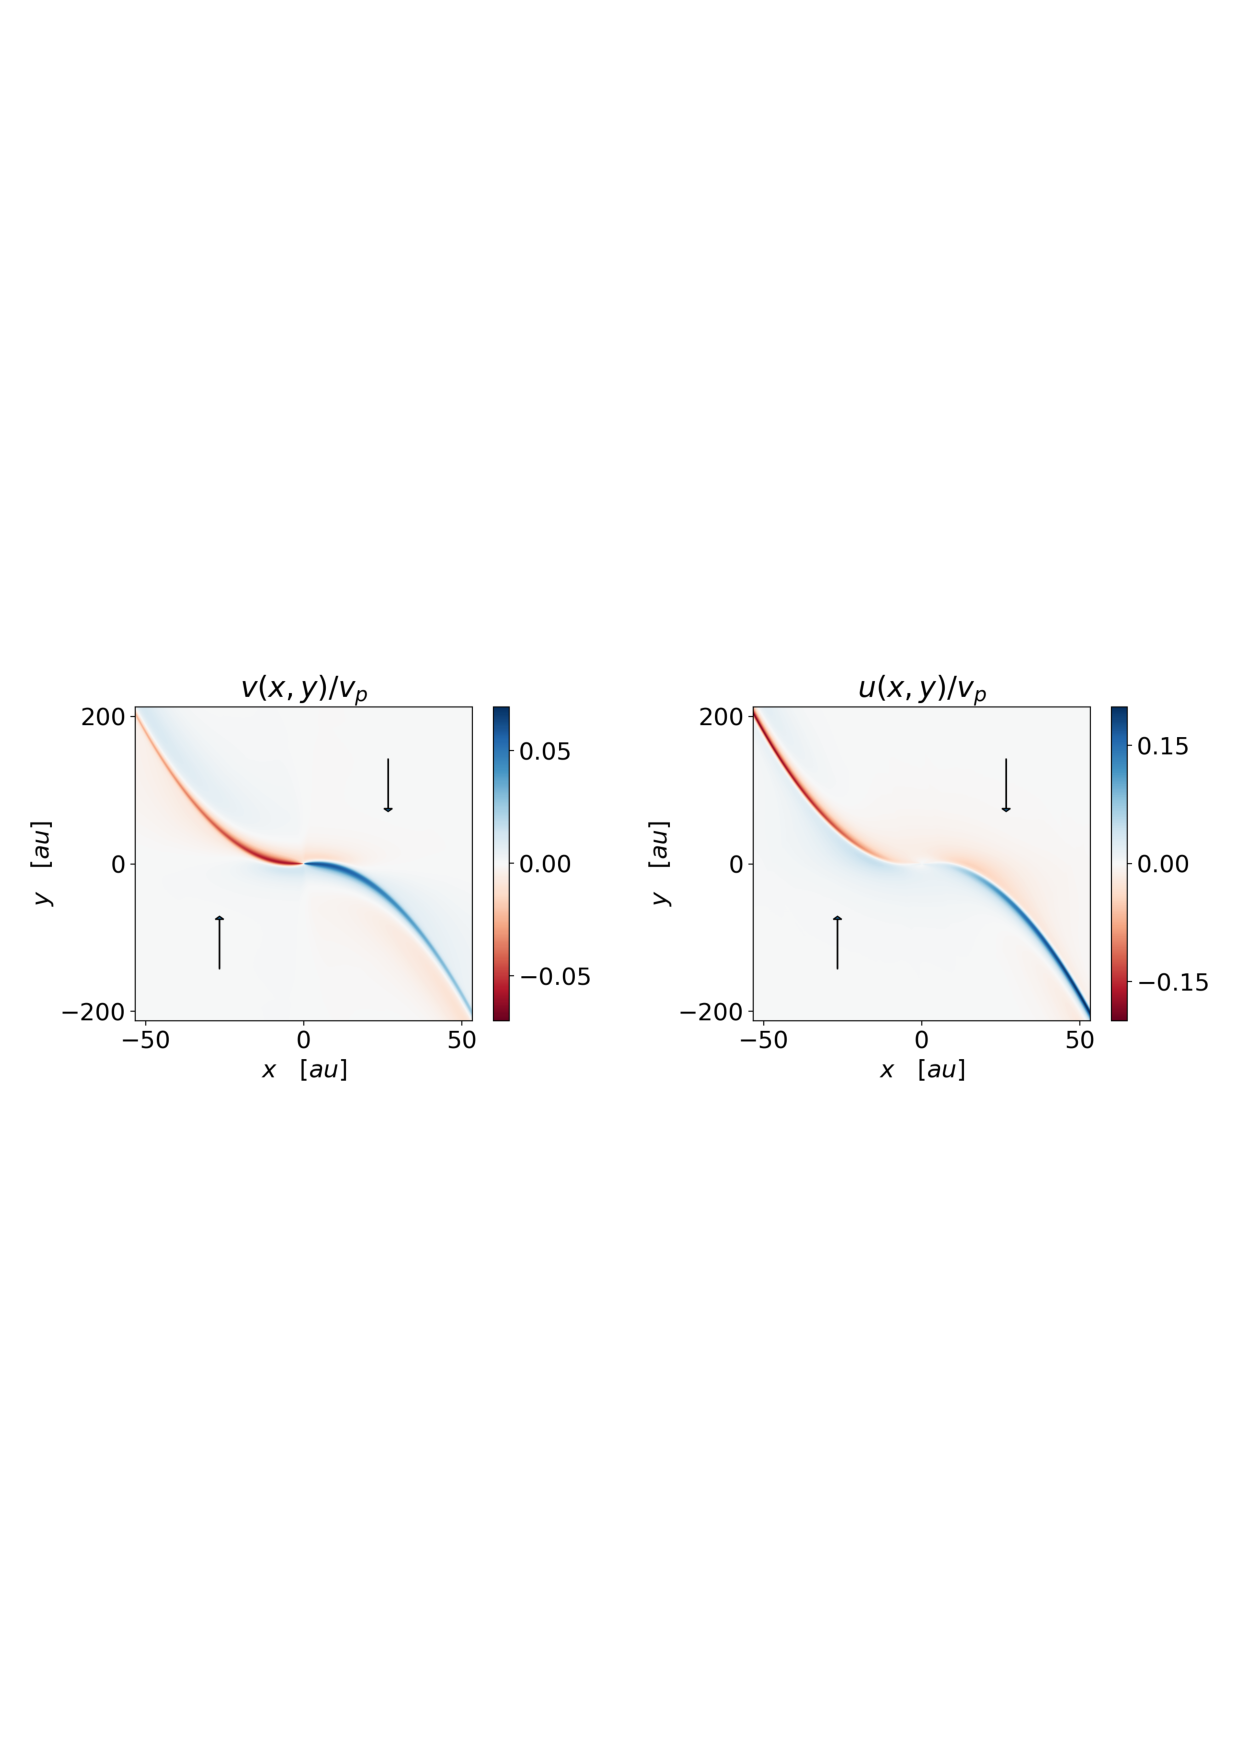
\includegraphics[width = 0.95\textwidth]{figures/linear_box_bollati.pdf}
    \caption{Linear azimuthal (left) and radial (right) velocity perturbations $v$ and $u$ centred on the planet in local cartesian coordinates as defined in equations \ref{eq:local_x} and \ref{eq:local_y}, and calculated by \citet{bollati2021}. The velocity is given in units of $v_{\rm p} = \Omega_{\rm K}(r_{\rm p})$, and the arrows denote the direction of the shearing bulk gas flow in a frame centred on the planet.}
    \label{fig:lin_box_bollati}
\end{figure}

Unlike \citet{bollati2021}, we do not include the linear regime results as a square box in the global solution.
Instead, we take seriously the transformation \ref{eq:local_y}, and interpret $y$ as an arc-length instead of a true Cartesian coordinate, giving us a \textit{linear annulus segment} instead of a \textit{linear square box} (we will from now on refer to the former simply as the \textit{linear box}).
Indeed, when the $\chi$ initial condition is extracted from the edge of the box, this is the treatment used for $y$.
It is therefore more honest to take this approach when mapping the linear solution onto the global grid, and has the added benefit of resulting in a more continuous solution.
In addition, we allow for separate variation of the height (angular extent) and width (radial extent) of the box.
This is motivated by considering that the box size was originally chosen as the Mach-1 length through an argument about resonance location (see section \ref{sec:linear_wake_excitation}).
Since these locations are constant as $\phi$ varies, it is perfectly acceptable to extent the linear regime in the angular direction.
The caveat to this is that the linear solution was derived in the shearing sheet approximation where the global geometry of the disk is not considered.
The curvature of the $y$ coordinate becomes more extreme as the box size increases angularly.
By default, \textsc{wakeflow} chooses the angular extent of the box to be the same as the radial extent, with a height of $4H_{\rm p}/3$.

\subsection{Transformations} \label{sec:transformations}

To perform transformation between the physical coordinates and $(t,\eta)$ space in calculating our models, we apply the general forms of the transformations \ref{eq:g} -- \ref{eq:eta} to so-called \textit{power-law disks} where the sound speed and surface density are parameterised as
\begin{align}
    c(r) = c_{\rm p} \left(\frac{r}{r_{\rm p}}\right)^{-q}; \quad \Sigma(r) = \Sigma_{\rm p} \left(\frac{r}{r_{\rm p}}\right)^{-\delta},
\end{align}
where $c_{\rm p}$ and $\Sigma_{\rm p}$ are the sound speed and surface density at $r_{\rm p}$.
Assuming also that $\Omega=\Omega_{\rm K}$, then equation \ref{eq:phi_wake} becomes \citep{rafikov2002a}
\begin{align}
    \phi_{\rm wake}(r) = \phi_{\rm p} + {\rm sgn} \left( r - r_{\rm p} \right) \frac{r_{\rm p}}{H_{\rm p}} \left[ \frac{2}{2q-1} \left(\frac{r}{r_{\rm p}}\right)^{q-\frac{1}{2}} - \frac{1}{q+1} \left(\frac{r}{r_{\rm p}}\right)^{q+1} - \frac{3}{\left(2q-1\right)\left(q+1\right)} \right].
\end{align}
Additionally, the Keplerian rotation implies $|2A| = 3\Omega/2 = 3c/2H$ and so the Mach-1 length becomes
\begin{align}
    l_{\rm p} = \frac{2H}{3},
\end{align}
and so the $\eta$ transformation \ref{eq:eta} reduces to 
\begin{align}
    \eta(r, \phi) = \frac{3 r_{\rm p}}{2 H_{\rm p}} \left[ \phi - \phi_{\rm wake} \right].
\end{align}
Additionally the $t$ transformation becomes \citep{rafikov2002a}
\begin{align}
    t(r) = \frac{3}{2^{5/4}} \left( \frac{r_{\rm p}}{H_{\rm p}} \right)^{\frac{5}{2}} \left| \int_1^{r/r_{\rm p}} |s^\frac{3}{2} - 1|^\frac{3}{2} s^{\frac{5q+\delta}{2}-\frac{11}{4}}\, ds \right|, \label{eq:t_power}
\end{align}
where explicitly the $g$ function is given by \citep{bollati2021}
\begin{align}
    g(r) = 2^{1/4} \left( \frac{r_{\rm p}}{H_{\rm p}} \right)^{\frac{1}{2}} \frac{\left( \frac{r}{r_{\rm p}} \right)^{\frac{5}{4} - \frac{\delta + 3q}{2}}}{\left| 1 - \left(\frac{r}{r_{\rm p}}\right)^\frac{3}{2} \right|^\frac{1}{2}} \label{eq:g_power}
\end{align}
This gives us all the tools we need to map from $(r,\phi)$ space to $(t,\eta)$ space in a Keplerian power law disk.
These are the forms of the transformations used by \textsc{wakeflow}.
We are therefore implicitly assuming that the unperturbed rotation profile is well approximated as Keplerian in the mid-plane, which is reasonable since the correction is of order $\left(H/r\right)^2$.

Unlike in \citet{goodman2001,rafikov2002a,bollati2021} we do not use approximate forms of the transformations that hold nearby the planet in the shearing sheet approximation to extract the initial condition for the Burger's evolution.
We found that the approximate transformation for $\eta$ \citep[equations 35 in][]{rafikov2002a} shifted the wake profile in $\eta$ by a few percent, leading to a discontinuity in the solution at the interface between the linear and non-linear regimes.
The approximate $t$ transformation has a similar effect although it is much smaller.
For this reason we always use the exact transformations as listed above.

Previously \citet{bollati2021} assumed that the initial condition for the inner ($r<r_{\rm p}$) and outer ($r>r_{\rm p}$) wake propagation were identical and so solved only the outer wake case and copied the solution for the inner wake.
This approximation does not hold well except for very small values of $(H/r)_{\rm p}$, as the radial extent of the box results in different $t$ coordinates at the inner and outer edge of the box in general.
For this reason we instead solve separately the inner and outer wake propagation, taking the appropriate initial condition for each (\citeauthor{fasanoinprep.}, in prep.).

After Burger's equation is solved numerically, the solution must be mapped from $\chi(t,\eta)$ to $\chi(r,\phi)$.
Since $t(r)$ is not invertible, we instead find the $(t,\eta)$ coordinates of every point on the solution grid $(r,\phi)$ and interpolate from the Burger's solution in $t,\eta$ space.
We therefore must evaluate the $t(r)$ and $\eta(r,\phi)$ transformations $N$ times, where $N$ is the number of points in the grid.
The $\eta$ transformation is easily vectorised since it is a simply algebraic expression, however the $t(r)$ transformation \ref{eq:t_power} involves an integral which naively must be evaluated $N$ times.
This approach is very inefficient, since the integral in the transformation does not actually depend on $r$, merely the end point does.
Re-evaluating the integral each time therefore often involves integrating over the same interval very many times.
In \textsc{wakeflow} we instead convert mapping $r\rightarrow t$ into an initial value problem (IVP).
Since the integrands of equation \ref{eq:t} is independent of r, we can convert equation \ref{eq:t} into an ordinary differential equation with an appropriate initial condition
\begin{align}
    \frac{dt(s)}{ds} = \frac{r_{\rm p}}{l_{\rm p}} \left[ \frac{\Omega(s) - \Omega_{\rm p}}{c_0(s) g(s)} \right]; \quad \, t(r_{\rm p}) = 0.
\end{align}
where obtaining $t(r)$ from the solution $t(s)$ is simply a matter of taking $s=r$.
Applying this analysis to the $t$ transformation for a power law disk \ref{eq:t_power} we obtain 
\begin{align}
    \frac{dt(s)}{ds} = \frac{3}{2^{5/4}} \left( \frac{r_{\rm p}}{H_{\rm p}} \right)^{\frac{5}{2}} \left| |s^\frac{3}{2} - 1|^\frac{3}{2} s^{\frac{5q+\delta}{2}-\frac{11}{4}} \right|; \quad t(1)=0, \label{eq:t_power_IVP}
\end{align}
and $t(r)$ is obtained from the solution taking $s=r/r_{\rm p}$.
\textsc{wakeflow} calculates the $t$ coordinates of the grid points by solving the IVP \ref{eq:t_power_IVP} using the \textsc{SciPy} function \textit{integrate.odeint} \citep{virtanen2020}.

\subsection{The High Mass Regime} \label{sec:high_mass}

Before we discuss our final improvement to the semi-analytic models, a higher order accuracy mapping from $\chi$ to the velocity perturbations $u$ and $v$, we will briefly address the question of the validity of the semi-analytic wake solution for planet masses of order $M_{\rm th}$.
While \citet{cimerman2021} performed a numerical validation of the models for the mass range $\le \frac{1}{2} M_{\rm th}$, we are particularly interested in more massive planets.
In the upcoming paper \citeauthor{fasanoinprep.} (in prep.) we will present detailed comparisons between simulations performed with the smoothed particle hydrodynamics (SPH) code \textsc{phantom} \citep{price2018} and the semi-analytic models, in the high mass regime with planet masses $\gtrsim M_{\rm th}$.
We will summarise the main findings of that work here.

For planet masses greater than $M_{\rm th}$, the linear solution is no longer valid as the wake should shock before it is fully formed \citep{goodman2001}.
It is then impossible to spatially separate the wake evolution neatly into the linear and non-linear regimes.
Ignoring this issue and calculating the semi-analytic models as usual introduces a few issues that we found to be discrepant with the simulation results.
Firstly, the wake structure in the linear box does not match that of the simulated models, and over-predicts the amplitude of the perturbations.
A sharp spatial discontinuity is also formed at the boundary between the linear and non-linear regimes, since the very large linear perturbation initial condition results in very rapid shock formation in the non-linear regime.
This discontinuity is visible in Figure \ref{fig:2_0mth}, and is more extreme for the radial velocity perturbations than for the azimuthal velocity or density perturbations.
There is also an additional continuity over the box edge in the amplitude of the velocity perturbations, with the perturbation just outside the linear box being far greater than that just inside.

\begin{figure}[H]
    \centering
    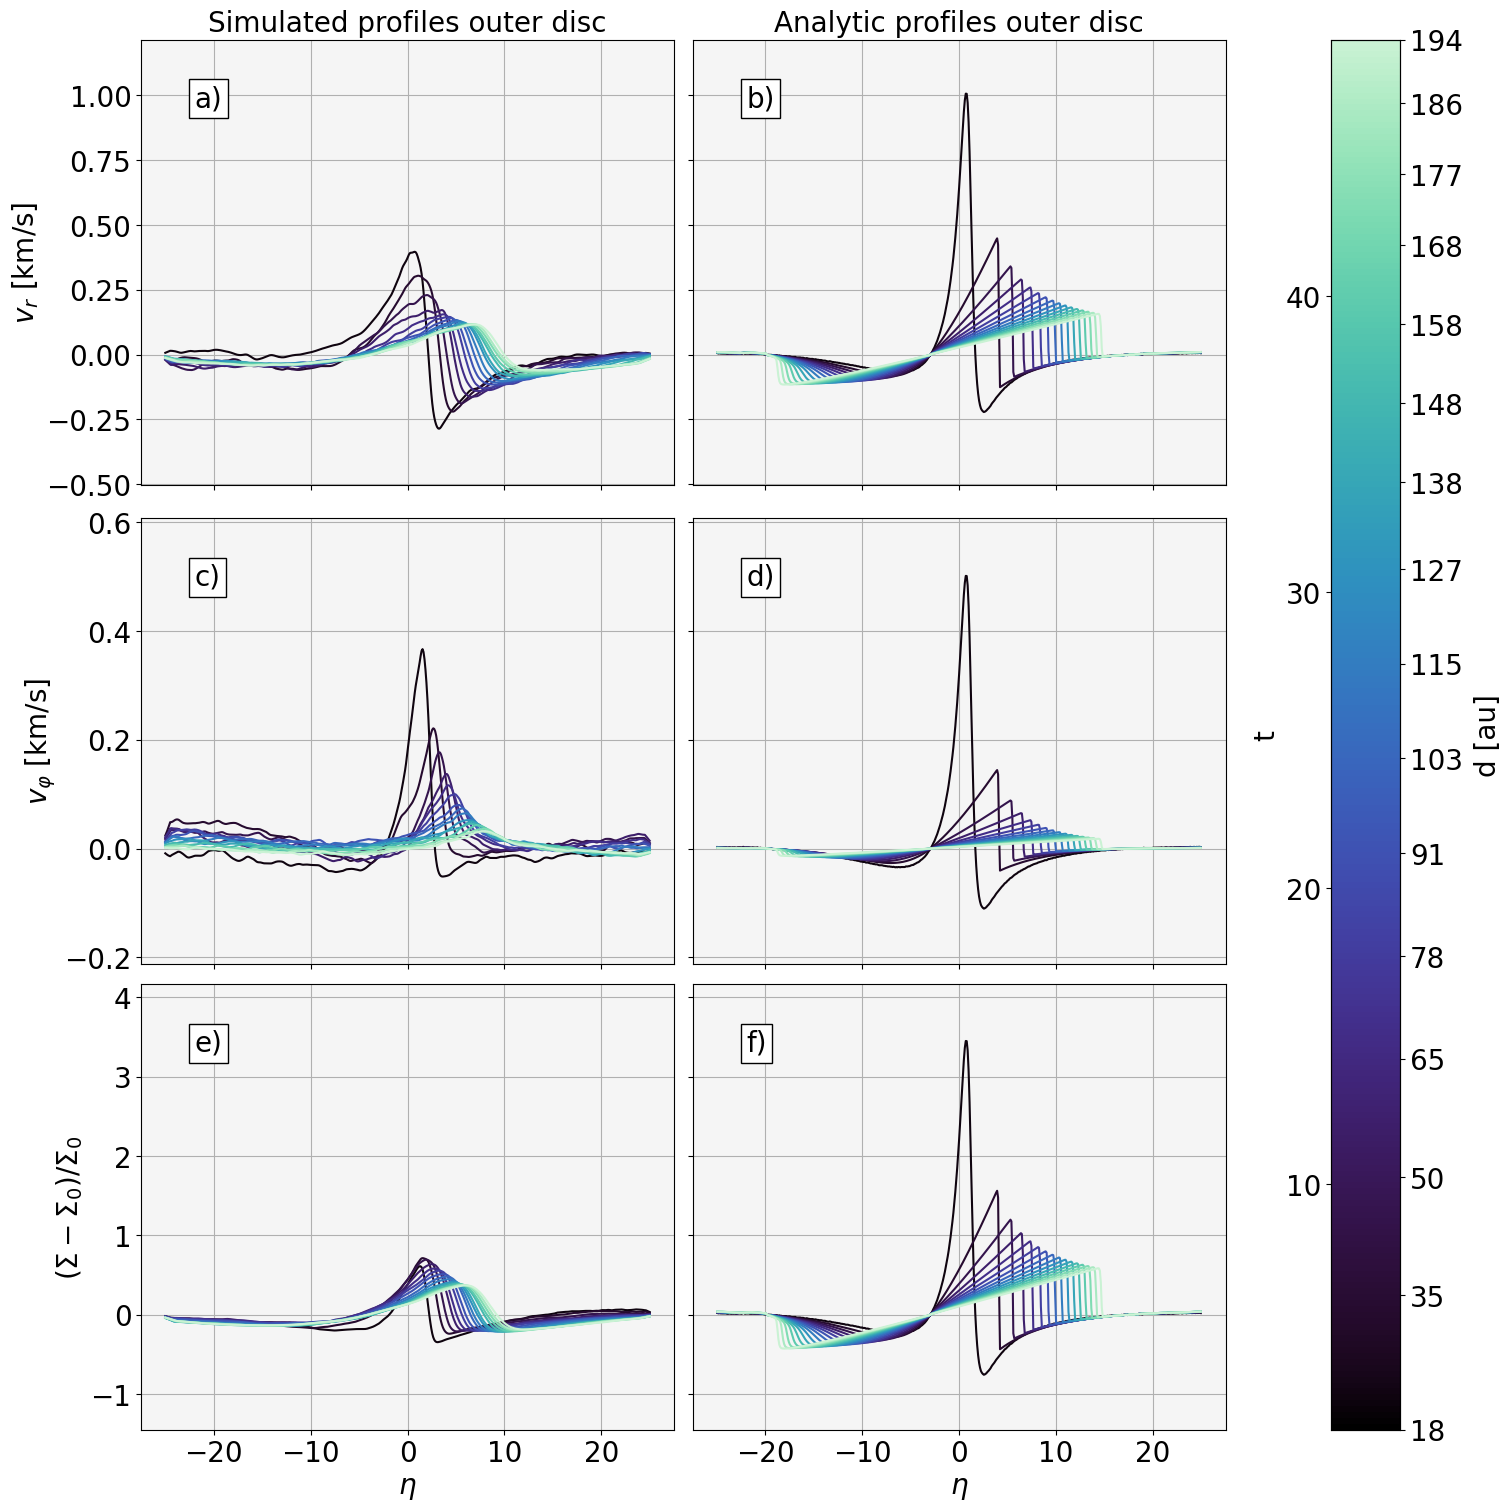
\includegraphics[width = 0.98\textwidth]{figures/comp_as_prof_out_high.png}
    \caption{Comparison between SPH (left) and semi-analytic (right) solutions for the perturbations induced by a $3.87 \, M_{\rm th}$ planet with orbital radius $r_{\rm p}=95.7 \, \mathrm{au}$. Wake profiles taken as slices of constant $t$, or equivalently $r$ are shown. The radial velocity, azimuthal velocity and density perturbations shown from top to bottom. The colourbar indicates the $t$ coordinate for each profile, as well as the physical distance $d$ from the planet location. Figure taken from \citeauthor{fasanoinprep.} (in prep.).}
    \label{fig:profile_comparison}
\end{figure}

However, moving away from the planet and deeper into the non-linear regime the agreement between the analytical and simulated models improves.
Figure \ref{fig:profile_comparison} shows the outer wake profile as it evolves in $t$ for $3.87 \, M_{\rm th}$, compared between both models.
Remarkably, the accuracy in the non-linear regime seems to improve as $t$ increases.
The amplitude for each of the perturbations is in good agreement between the models after the wake was propagated only a few tens of $\mathrm{au}$ from the planet location.
The shocks produced by the inviscid Burger's equation evolution are however steeper than those found in the SPH model, like due to the artificial viscosity present in the simulation \citep{lodato2010}.
The wake profiles are more extended in $\eta$ in the analytics, but we do not seem to recover the over-damping found in the low mass regime by \citet{cimerman2021}.
The position of the outer shock in density, and so the shape of the wake, is also different between the models.
This is not surprising as the pitch angle of the spiral increases and deviates from the linear shape used in the analytics \ref{eq:phi_wake} for high mass planets \cite{zhu2015}.
It may be possible to calibrate for this increase in pitch angle from non-linear effects, see section 5.2 of \citet{cimerman2021} for more details.

The apparent accuracy of the solution in the semi-analytical model far from the planet in the high mass case is perhaps not surprising when considered in the context of the existence of the asymptotic solution given in section \ref{sec:asymptotic_N_wave}.
The more massive planets result in faster shock formation in the Burger's equation evolution, and so it makes at least qualitative sense that the asymptotic solution may also become valid earlier.
The agreement between the analytics and simulations for $t \gtrsim 10$ may therefore reflect that the solution quickly becomes independent of the initial condition, and that the asymptotic scaling in $\chi$ holds well for high planets resulting in the correct non-linear behaviour at some distance from the planet.
We defer further discussions of accuracy, including a full parameter study and a preliminary calibration of the semi-analytic method, to \citeauthor{fasanoinprep.} (in prep.).

\subsection{Velocity Perturbations} \label{sec:velocity_perts}

Following the method of \citet{bollati2021} to calculate the velocity perturbations in the non-linear regime results in a discontinuous solution at the edge of the linear box, as the amplitude of the velocity perturbations for $t>t_0$ is smaller than that at the start of the non-linear solution where $t-t_0$ is small\footnote{Recall that $t_0$ is the $t$ coordinate at the transition between the linear and non-linear regimes.} (\citeauthor{fasanoinprep.}, in prep).
To investigate this discontinuity in velocity amplitude we re-derive the mapping from $\chi$ to $u$ and $v$ derived by \citet{rafikov2002a} and \citet{bollati2021}.
As we saw in section \ref{sec:nonlinear_evolution} the conservation of the Riemann invariant $R_+$ gives for the radial velocity perturbation
\begin{align}
    u = 2\frac{c_0-c}{\gamma - 1}=-2\frac{c_0}{\gamma + 1} \psi, \label{eq:u_rafikov}
\end{align}
where we define $\psi$ as
\begin{align}
    \psi = \frac{\gamma+1}{\gamma-1} \frac{c - c_0}{c_0},
\end{align}
which is the sound speed perturbation with a constant scale factor. Following \citet{rafikov2002a}, we then derive an expression for $\psi$ in terms of the density perturbation $\chi$ by assuming that the gas obeys a locally polytropic equation of state given by 
\begin{align}
    P = P_0(r) \left[ \frac{\Sigma}{\Sigma_0(r)} \right]^\gamma. \label{eq:poly_EOS}
\end{align}
The sound speed is then
\begin{align}
    c^2 = \frac{\partial P}{\partial \Sigma} = c_0^2(r) \left[ \frac{\Sigma}{\Sigma_0(r)} \right]^{\gamma-1}.
\end{align}
Rafikov then finds a relation between the density and sound speed perturbations, to second order in $\psi$, by expanding the above expression. 
This yields
\begin{align}
    \frac{\Sigma - \Sigma_0}{\Sigma_0} = \frac{2}{\gamma + 1}\psi + \frac{3 - \gamma}{\left( \gamma + 1  \right)^2} \psi^2 + \mathcal{O}(\psi^3). \label{eq:psi_exp}
\end{align}
Taking this expression to first order only, we write $u$ in terms of the density perturbation, and then in terms of $\chi$ by substituting equation \ref{eq:chi}. 
\begin{align}
    u = - c_0 \frac{\Sigma - \Sigma_0}{\Sigma_0} = -2 \frac{c_0}{\gamma + 1} \frac{\chi}{g(r)}. \label{eq:ap_rad_vel}
\end{align}
Similarly, \citet{rafikov2002a} finds the azimuthal velocity as
\begin{align}
    v \approx -2 \frac{c_0^2}{\Delta\Omega r} \frac{1}{\gamma + 1} \psi, \label{eq:v_rafikov}
\end{align}
giving to first order in $\psi$
\begin{align}
    v \approx - \frac{c_0^2}{\Delta \Omega r} \frac{\Sigma - \Sigma_0}{\Sigma_0} = - \frac{2}{\gamma + 1} \frac{c_0^2}{\Delta \Omega r} \frac{\chi}{g(r)}. \label{eq:ap_az_vel}
\end{align}
equations \ref{eq:ap_rad_vel} and \ref{eq:ap_az_vel} are the expressions used in \citet{bollati2021} to calculate the velocity perturbations in the non-linear regime. 
Since these are only accurate to first order in $\psi$, the assumption is made that $\psi \ll 1$, which is the weak shock approximation introduced in section \ref{sec:nonlinear_evolution}.
Since we are in particular interested in the velocity perturbations in the context of kinematics, and in planet masses comparable to the thermal mass, we should check if the assumption that $\psi \ll 1$ still holds for more planets in the high mass regime.

We can derive an \textit{exact} expression for $\psi$ in terms of the density perturbation simply by rearranging equation \ref{eq:poly_EOS}. We find
\begin{align}
    \psi = \frac{\gamma + 1}{\gamma - 1} \left[ \left( \frac{\Sigma-\Sigma_0}{\Sigma_0} +1  \right)^{(\psi-1)/2}  -1 \right],
\end{align}
which can be written equivalently in terms of $\chi$ using equation \ref{eq:chi} giving
\begin{align}
    \psi = \frac{\gamma + 1}{\gamma - 1} \left[ \left( \frac{2}{\gamma + 1} \frac{\chi}{g(r)} +1  \right)^{(\psi-1)/2} -1 \right]. \label{eq:psi_exact}
\end{align}
We will use equation \ref{eq:psi_exact} to check the aforementioned assumption that $\psi \ll 1$ in the non-linear regime solution. 
We construct three \textsc{wakeflow} models using dimensionless units, with embedded planet masses of $0.5, 1.0$ and $2.0 \, M_{\rm{th}}$ respectively, all placed in orbit around a $1 \, M_{\rm{\odot}}$ star at an orbital radius of $r=1$. 
For all models, we choose $p=2.25$ and $q=0.25$ such that $\Sigma \propto r^{-1}$, and an aspect ratio $H/r=0.1$ at $r=1$. 
Figure \ref{fig:psi_comparison} shows the values of $\psi$ for each of these models, and demonstrates that even for the lowest planet mass model the value of $\psi$ nearby the planet is as large as $\sim \hspace{-0.23em} 0.6$ and so the second order terms will clearly be important even in this case. 
For masses $\ge \hspace{-0.23em} M_\mathrm{th}$ the problem is even worse, as there are regions where $\psi \gtrsim 1$ causing the expansion given in equation \ref{eq:psi_exp} to diverge.

\begin{figure}
    \centering
    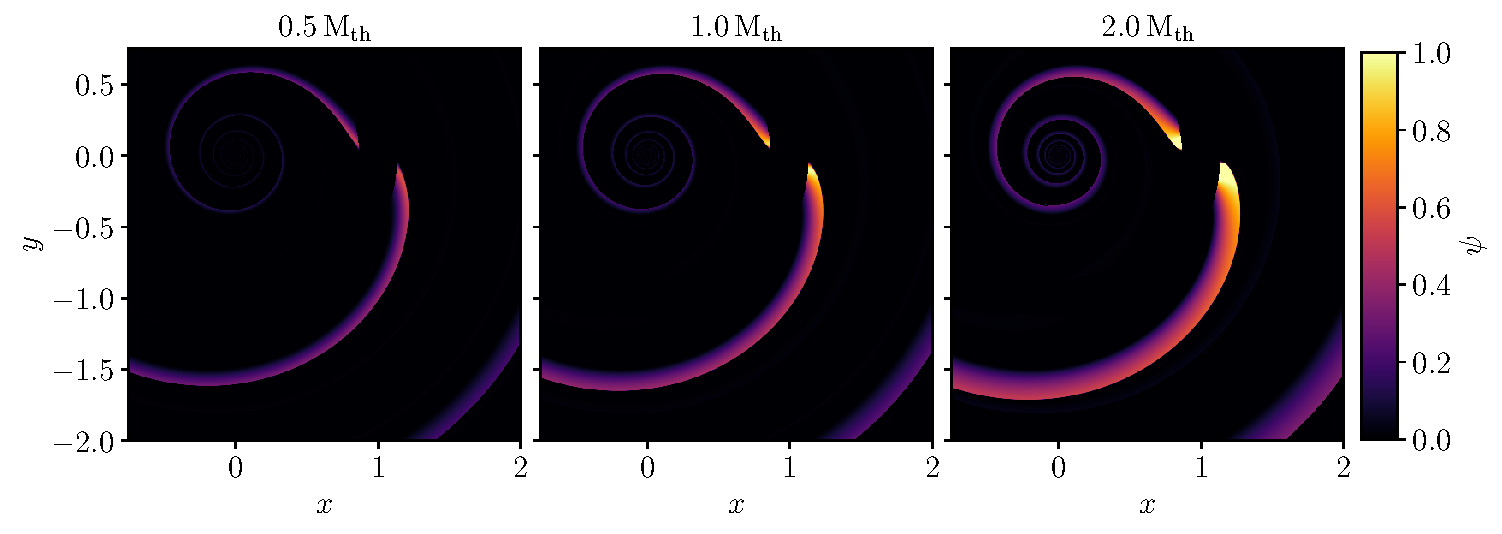
\includegraphics[width = 0.98\textwidth]{figures/psi 2.pdf}
    \caption{Comparison of the values of $\psi$ calculated from equation \ref{eq:psi_exact} for three \textsc{wakeflow} models with planet masses of $0.5, 1.0$ and $2.0 \, M_{\rm{th}}$ respectively. Clearly one cannot assume that $\psi \ll 1$ even for the lowest mass model, especially nearby the planet. For the two larger masses, there are even regions where $\psi > 1$.}
    \label{fig:psi_comparison}
\end{figure}

The choice of taking \ref{eq:psi_exp} to first order is justified in \citet{bollati2021} by noting that terms proportional to $\psi^2$ are discarded in the derivation of the Burgers evolution \ref{eq:burgers}, and thus also in the calculation of $\chi$ from which $u$ and $v$ are calculated.
The $u$ and $v$ calculated by their method are thus those that are consistent with the solution to Burger's equation \ref{eq:burgers}. 
However it is not clear that this gives the most physically reasonable results.
The argument for the velocities follows by relating the sound speed perturbation to the density perturbation through the equation of state \ref{eq:poly_EOS}.
However it is not clear that truncating the equation of state for density perturbations calculation \textit{necessitates} that the same truncation must be performed to find physically realistic velocity perturbations.

In order to obtain velocity perturbations that more closely match hydrodynamical simulations, and to reduce the amplitude discontinuity over the box, we derived expressions for both $u$ and $v$ as functions of $\chi$ without truncating the equation of state to first order in $\psi$. 
This is as simple as substituting equation \ref{eq:psi_exact} into equations \ref{eq:u_rafikov} and \ref{eq:v_rafikov}, yielding
\begin{align}
    u(\chi) &= -2 \frac{c_0}{\gamma - 1} \left[ \left( \frac{2}{\gamma + 1} \frac{\chi}{g(r)} +1  \right)^{(\psi-1)/2} -1 \right] \label{eq:u_chi_new} \\
    v(\chi) &\approx \frac{c_0}{\Delta\Omega r} u (\chi). \label{eq:v_chi_new} 
\end{align}
\begin{figure}
    \centering
    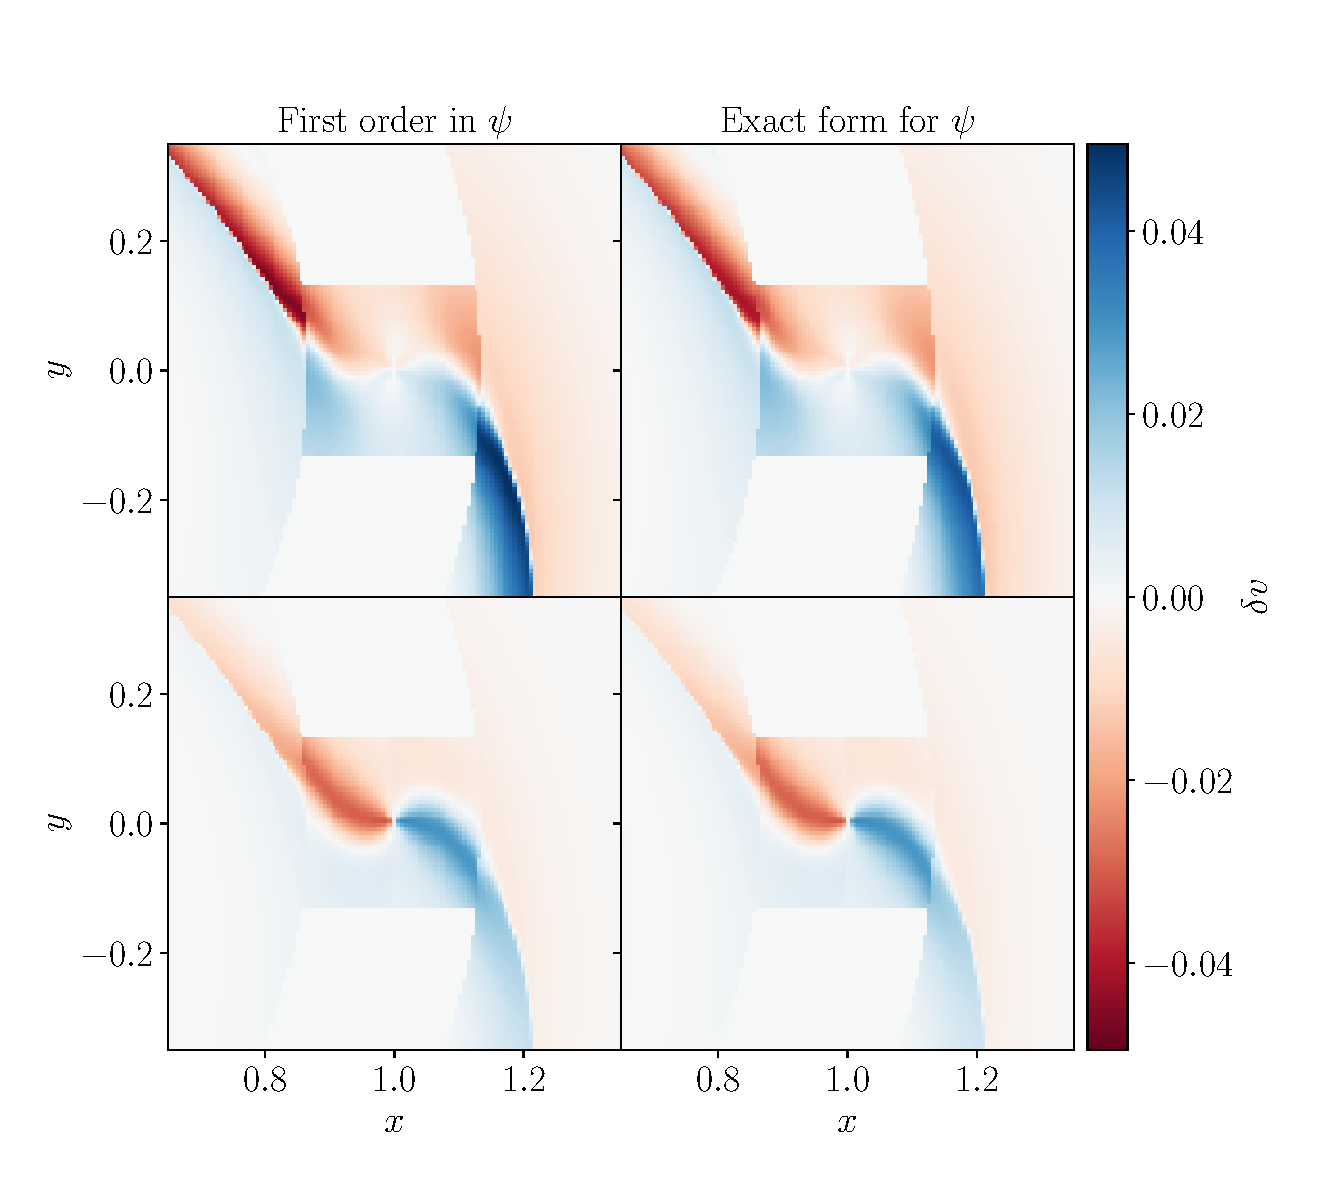
\includegraphics[width = 0.7\textwidth]{figures/0_5_mth.pdf}
    \caption{Comparison of the velocity perturbations calculated in the non-linear regime between the method of \citet{bollati2021} which is first order accurate in $\psi$ (left), and by using equations \ref{eq:u_chi_new} and \ref{eq:v_chi_new} which use the exact form for $\psi$ (right). The dimensionless radial velocity and azimuthal velocities are shown in the top and bottom panels respectively. The planet mass used in the model is $0.5 \, M_{\rm th}$. We see that the amplitude discontinuity is improved somewhat for the radial velocities, and basically unaffected for the azimuthal velocities.}
    \label{fig:0_5mth}
\end{figure}
\begin{figure}
    \centering
    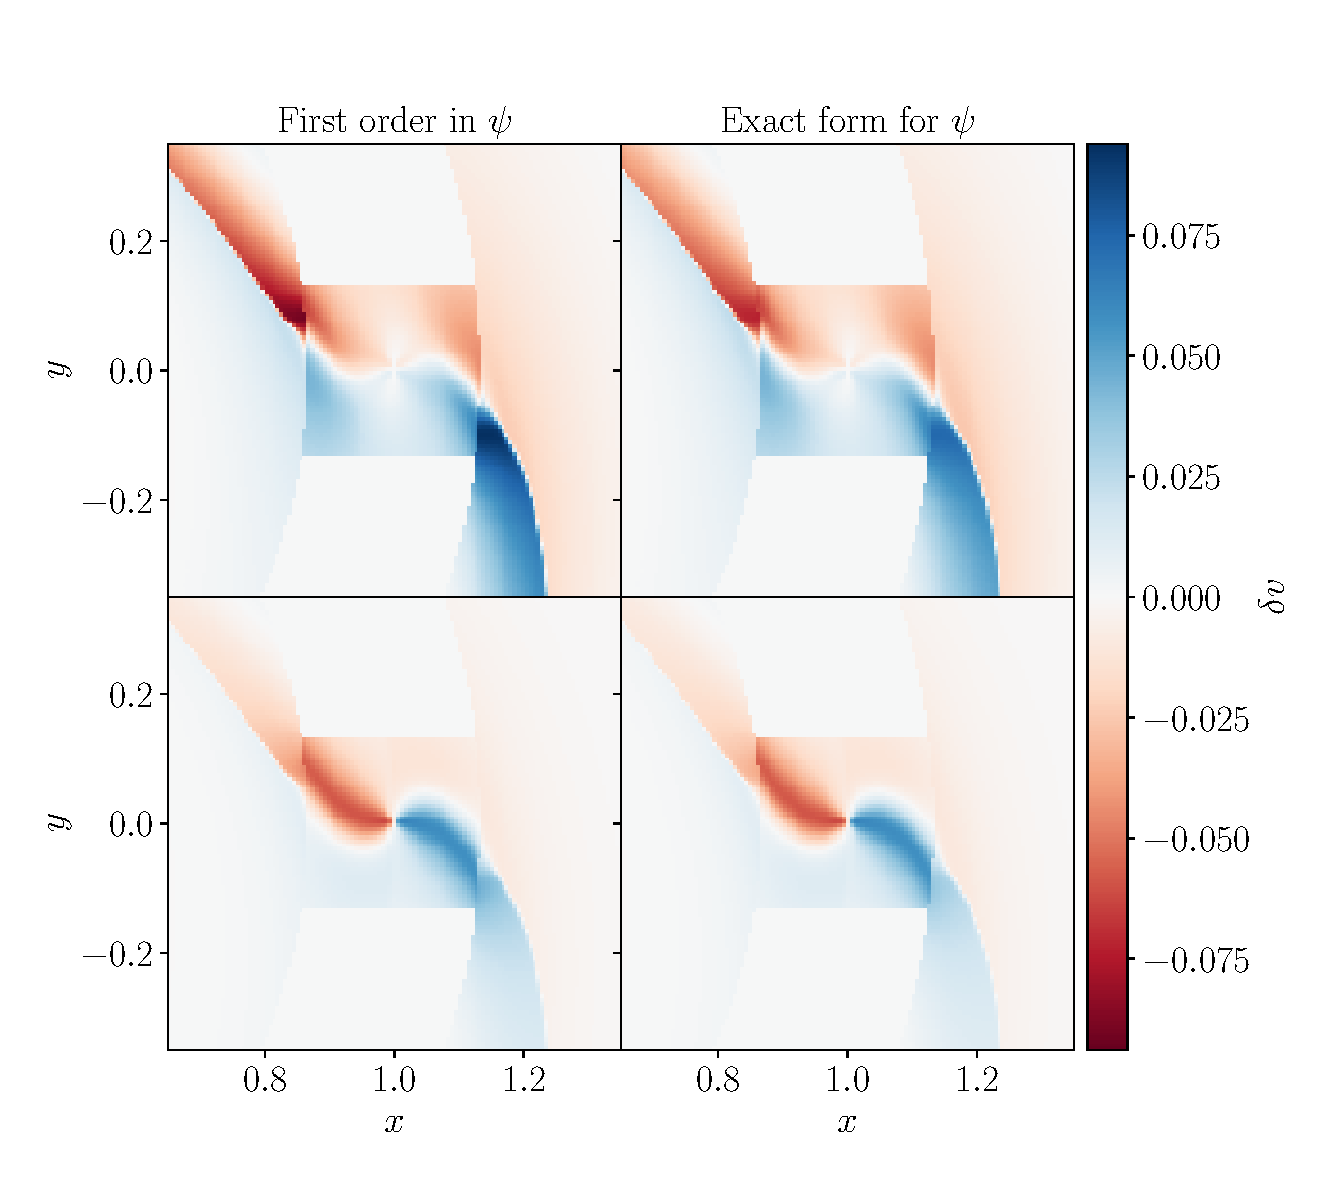
\includegraphics[width = 0.7\textwidth]{figures/1_0_mth.pdf}
    \caption{As in Figure \ref{fig:0_5mth}, except for a planet mass of $1.0 \, M_{\rm th}$. We see that the amplitude discontinuity is significantly improved for the radial velocities, but not for the azimuthal velocities.}
    \label{fig:1_0mth}
\end{figure}
\begin{figure}
    \centering
    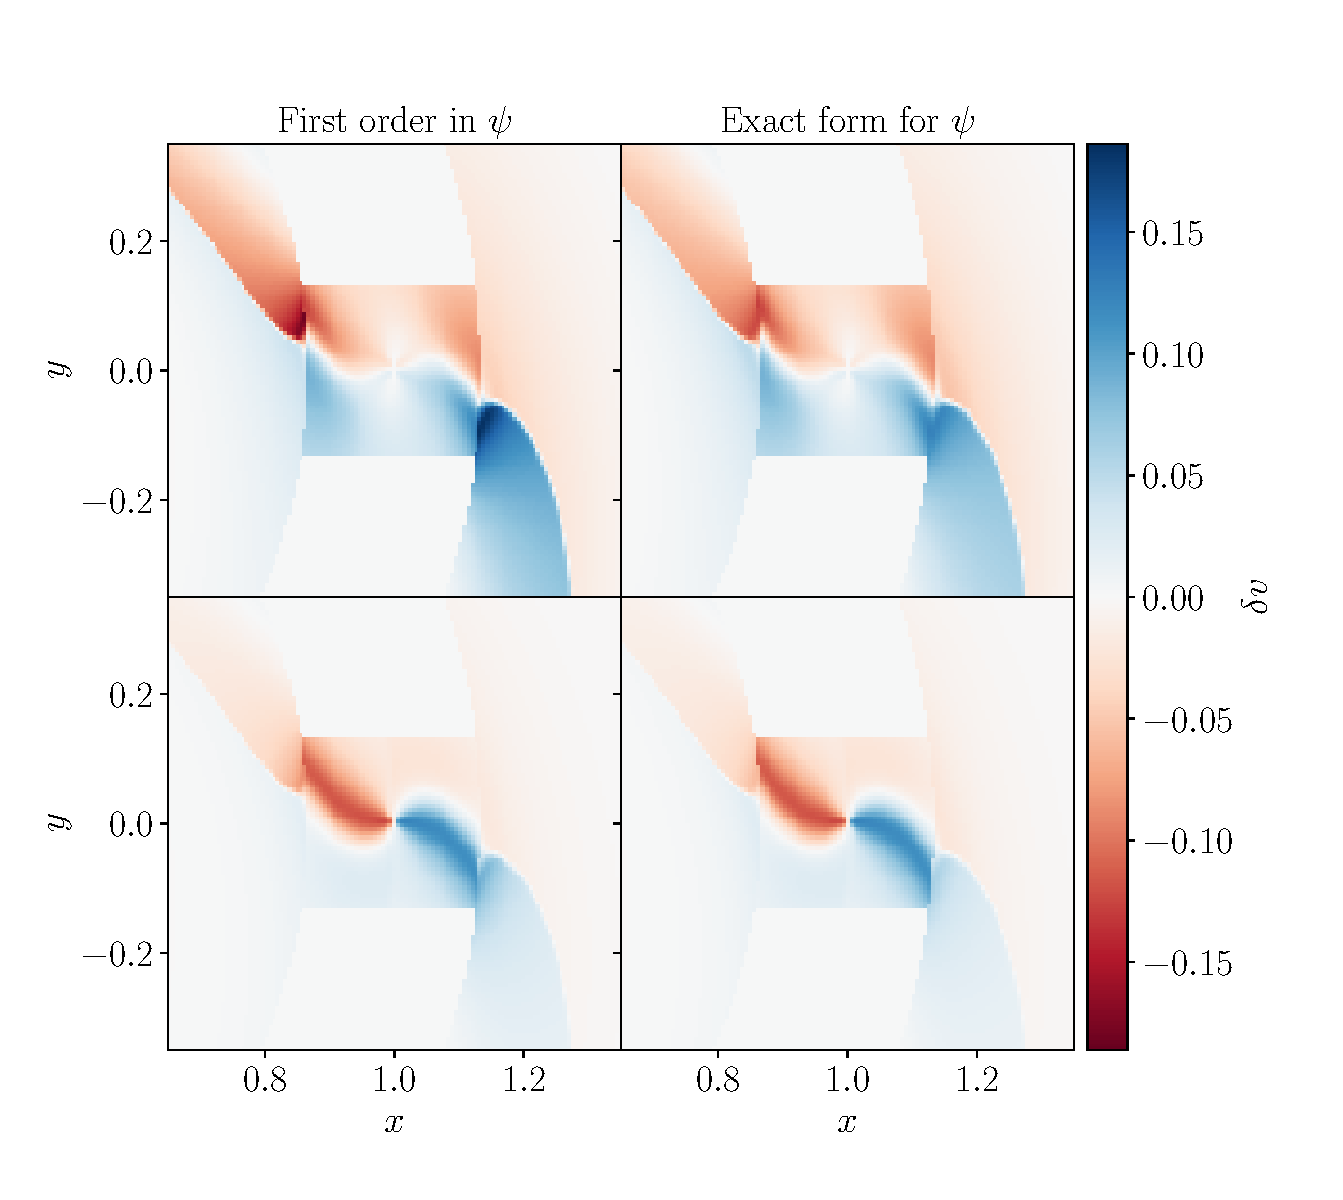
\includegraphics[width = 0.7\textwidth]{figures/2_0_mth.pdf}
    \caption{As in Figure \ref{fig:2_0mth}, except for a planet mass of $2.0 \, M_{\rm th}$. We see that the amplitude discontinuity is again significantly improved for the radial velocities, while unaffected or even slightly worse for the azimuthal velocities.}
    \label{fig:2_0mth}
\end{figure}
Figures \ref{fig:0_5mth},\ref{fig:1_0mth} and \ref{fig:2_0mth} show a comparison of the velocities calculated from the above with those calculated to first order in $\psi$, for planet masses of $0.5, 1.0$ and $2.0 \, M_{\rm th}$ respectively. 
These are the same models as those used to create Figure \ref{fig:psi_comparison}. 
The plots are centred on the planet location, and they show that even for the lowest mass case the amplitude discontinuity is improved significantly for the radial perturbations by the new extraction using equation \ref{eq:u_chi_new}. 
This affect is increasingly significant for the massive planets as can been seen in the $1.0$ and $2.0 \, M_{\rm th}$ cases. The azimuthal velocity case is however minimally affected. 
It is unclear why the radial perturbation is improved while the azimuthal perturbation is not.
However the derivation for $u(\psi)$ in \citet{rafikov2002a} comes from the conservation of the Riemann invariant $R_+$, while $v(\psi)$ is found in terms of $u$ by taking equation \ref{eq:phi_xi_v} and the terms $u \partial_\phi v$ and $u v / (\Delta \Omega r)$.
We conjecture that these terms are also important for larger mass planets, and that they could be responsible for the lack of improvement in the $v$ mapping.

Due to the reduction in the amplitude discontinuity, equations \ref{eq:u_chi_new} and \ref{eq:v_chi_new} are used to calculate the velocity perturbations in the non-linear regime in \textsc{wakeflow}. 

\section{Implications --- Non-Localised Velocity Kinks}

\citet{bollati2021} used 2D semi-analytic models to predict the morphology of velocity kinks that arise in kinematic observations \citep{pinte2018a} due to the velocity perturbations associated with the wake.
Figure \ref{fig:2D_kinks} shows the ``mock'' velocity channels that they generated by rotating the velocity perturbations to the line of sight for a disk inclined at $30^\circ$ from the sky plane.
They recover the abrupt sign reversal in velocity across the planet location first suggested by \citet{casassus2019}, the so-called \textit{Doppler flip}.
They also found that velocity kinks arise due to the intersection of the planet wake and the velocity channels, and that these kinks are spread throughout the disk.
Since at the time kinks were thought to be localised nearby the planet \citep{pinte2018a,pinte2019,pinte2020}, Bollati suggested that viscous damping may suppress the amplitude of the perturbations far from the planet.
As we will see in chapter \ref{ch:wake_mapping}, velocity kinks are in fact \textit{not} localised nearby the planet location.
High resolution kinematic observations allow for the mapping of the planet wake in the disk through spatially correlated kinks spread throughout the disk \citep{calcino2022,teague2022,verrios2022}

\begin{figure}%[H]
    \centering
    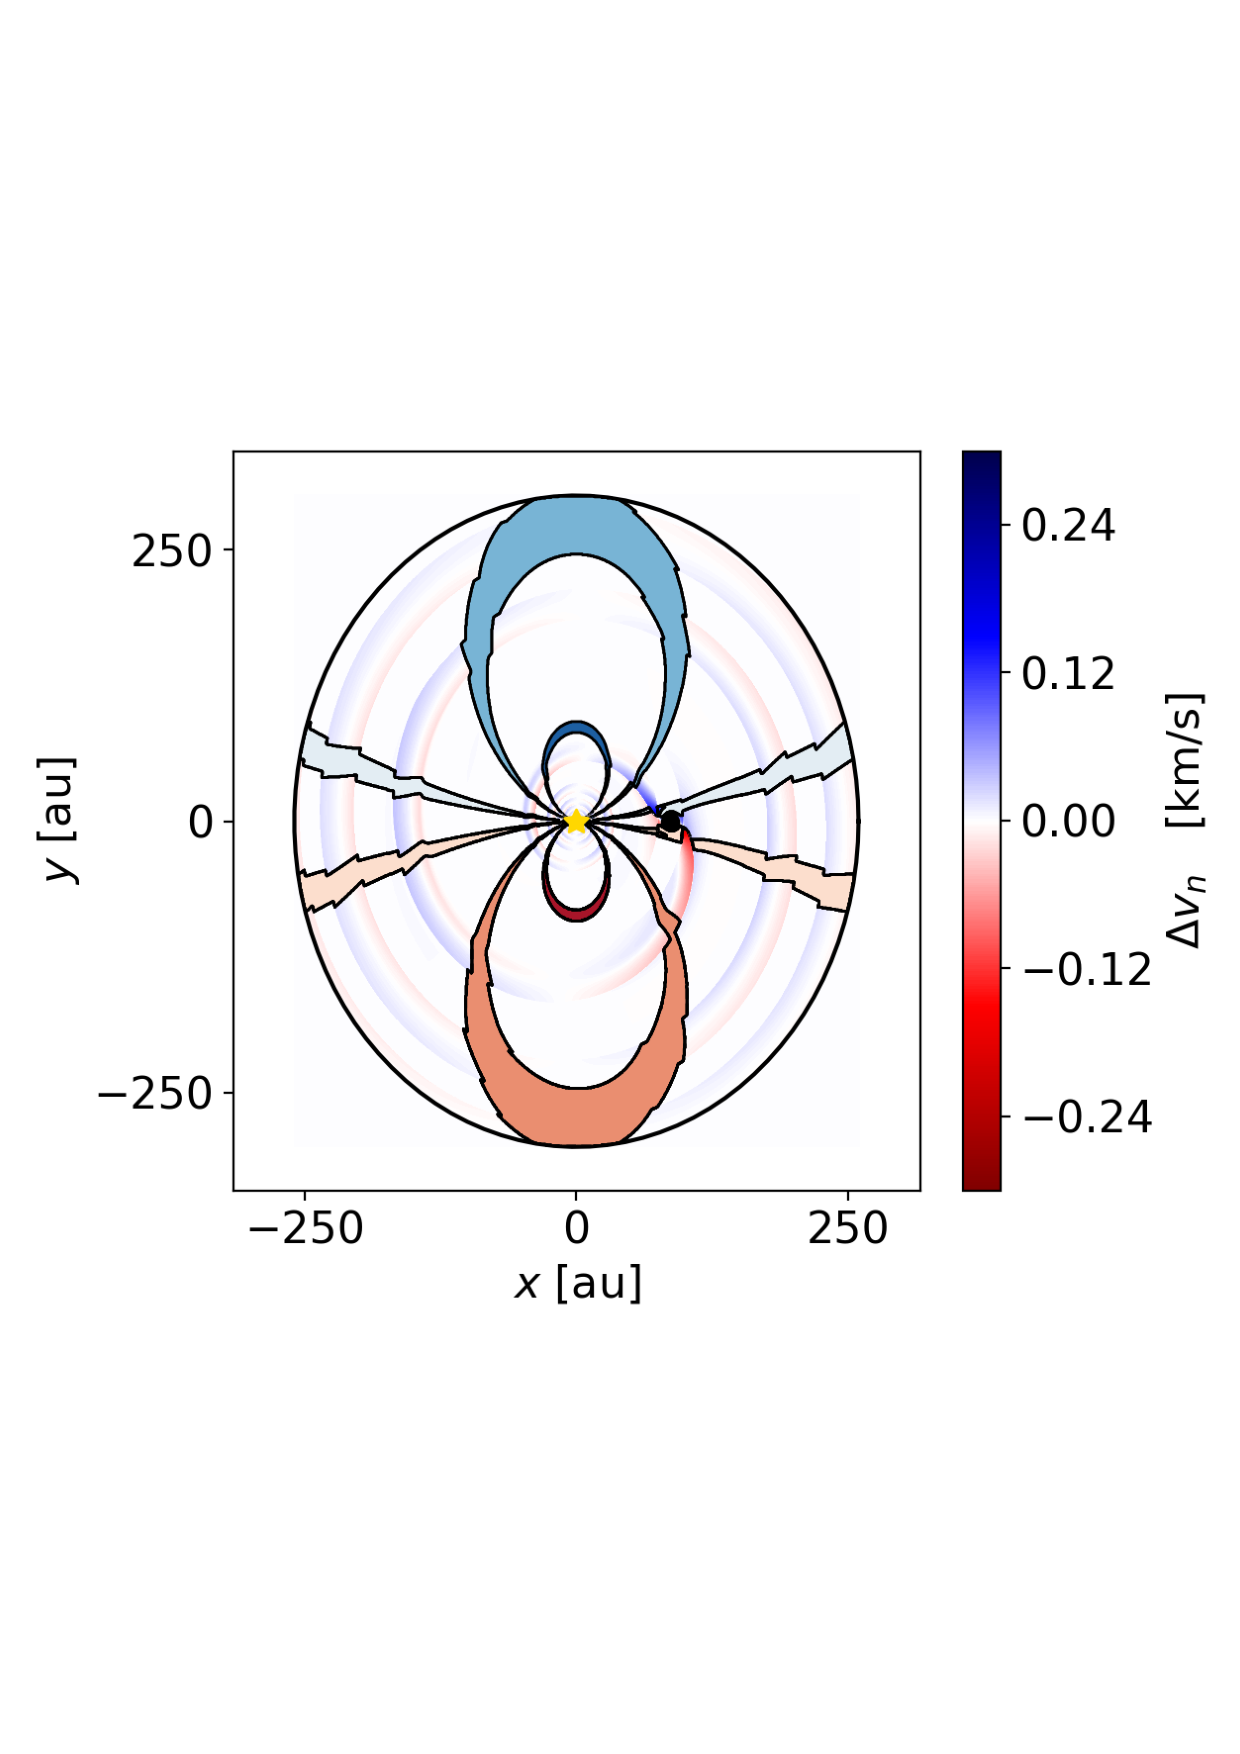
\includegraphics[width = 0.7\textwidth]{figures/bollati_2d_kinks.pdf}
    \caption{2 dimensional velocity channel maps generated from analytical models by \citet{bollati2021} for a disk inclined at $30^\circ$. The solid coloured bars represent velocity channels of width $\Delta v = 0.05 \, \mathrm{km/s}$, while the red and blue colouring gives the line-of-sight velocity perturbations. The planet and star locations are denoted by a black dot and yellow star symbol respectively. The chosen parameters for the model were $M_\star = 1\, M_\odot$, $M_{\rm p}=\mathrm{M_J}$, $r_{\rm p} = 100\, \mathrm{au}$ and $(H/r)_{\rm p}=0.1$.}
    \label{fig:2D_kinks}
\end{figure}

\section{Modelling the Kinematic Arc in HD~169142} \label{sec:hd169}

This section presents the semi-analytical modelling performed as a part of \citet{garg2022}, which is publicly available at \href{https://arxiv.org/abs/2207.02869}{\url{arXiv:2210.10248}}.

\subsection{Introduction}

HD~169142 is a disk-hosting Herbig Ae star located in the constellation of Sagittarius, at a distance of $117 \pm 4$ pc \citep{brown2016}.
The system's circumstellar disk appears almost face-on in the sky with an inclination of just $13^\circ$ \citep{raman2006,panic2008}.
The disk contains bright dust ring substructures at $\sim25$ au and $\sim65$ au, as well as a central cavity with radius $\sim22$ au.
These features have been observed through different tracers including scattered light \citep{quanz2013a,momose2015,pohl2017,bertrang2018} mid-infrared \citep{honda2012}, sub-millimetre with ALMA \citep{fedele2017,macias2019,perez2019} and centimetre with the Very Large Array \citep{osorio2014}.
The highest resolution of these studies showed that the outermost ring is actually three distinct rings separated by approximately $10$ au.
Various candidate point source detections have been made near the $r \approx 25$ au ring \citep{biller2014,reggiani2014,gratton2019}, but are disputed due to the possible confusion with disk material in their analyses \citep{ligi2018}.

This paper presents ALMA band 6 observations of the circumstellar disk around HD~169142.
We imaged the $^{12}$CO, $^{13}$CO and C$^{18}$O $J=2-1$ spectral lines at a resolution of $0.167 \, \mathrm{km/s}$, taking into account the Hanning Smoothing caused by the correlator.
The obtained angular resolutions of $0.07"$ and $0.1"$ allowed us resolve both density and kinematic substructures in the gas. Here, we will focus on the $^{12}$CO observations and the disk kinematics.

\subsection{Observations and Analysis}

We imaged the $J=2-1$ line transitions of $^{12}$CO, $^{13}$CO and C$^{18}$O using ALMA band~6 observations from projects [2015.1.00490.S] and [2016.1.00344.S].
For details of the self-calibration and data reduction process, see \citet{garg2022}.

From equation \ref{eq:rot_eq_full} we have the rotation velocity of the gas in a pressure-supported disk is given by 
\begin{align}
    \frac{v_{\rm gas}^2}{r} &= \frac{G M_\star r}{\left( r^2 + z^2  \right)^{3/2}} + \frac{1}{\rho_{\rm gas}} \partial_r P_{\rm gas}, \label{eq:gas_rotation}
\end{align}
where the first term is the typical Keplerian rotation and the second is the contribution by the radial pressure gradient.
As discussed in section \ref{sec:disk_rotation}, the second term typically results in sub-Keplerian motions.
To find kinematic substructures in the data, we wish remove the background motions of the disk associated with equation \ref{eq:gas_rotation} to isolate only the deviations from the bulk flow.
As a first step, we peak velocity $v_0$ maps by spectrally collapsing the data cube using the \textsc{Python} package \textsc{bettermoments} \citep{teague2018a}.
We chose specifically to use the \textit{Gaussian} method since it provides also the velocity error for each pixel $\delta v_0$ and has minimal statistical uncertainty \citep{yu2021}.

To obtain only the deviations from bulk rotation in $v_0$, we made use of the \textsc{Python} package \textsc{Eddy} \citep{teague2019}.
\textsc{Eddy} subtracts a best-fitting Keplerian rotation profile using a Markov Chain Monte Carlo (MCMC) method \citep{foreman-mackey2013}\footnote{The main point of using MCMC over a traditional optimisation method is to obtain the uncertainties in the best fitting parameters by estimating the posterior distribution. However, we found that the error-bars we obtained were too small to be physically realistic, and so in appendix C of \citet{garg2022} we provide a parameter study around the best fit to investigate the true uncertainty.}.
We fit for the disk position angle (PA), central star mass $M_\star$, central star pixel location $(x_0,y_0)$ and systemic velocity $v_{\rm syst}$.
For the MCMC, we used 250 walkers and ran for 10,000 steps.
The data used in the fit were also restricted to within $1.5"$ from the centre of the image, as outside of this region was noise dominated.
The inner $0.2"$, twice the beam width, was also exclude to avoid any bias resulting from beam smearing in the inner disk.
From fitting the $^{12}$CO data, we found best-fitting model parameters of $\mathrm{PA} = 5.33^\circ$, $M_\star = 1.47 \, \mathrm{M_\odot}$, and $v_{\rm syst} = 6.897 \, \mathrm{km/s}$.

To account for the pressure term of equation \ref{eq:gas_rotation}, we need the radial pressure gradient $\partial_r P_{\rm gas}(r)$.
Assuming an ideal gas equation of state, the pressure is given by 
\begin{align}
    P_{\rm gas}(r) = n_{\rm gas} k_{\rm B} T(r),
\end{align}
where $n_{\rm gas}$ is the gas number density, $k_{\rm B}$ is Boltzmann's constant and $T(r)$ is the temperature profile.
We calculated $n_{\rm gas}$ and $T(r)$ from the azimuthally averaged gas column density and brightness temperature profiles respectively, see \citet{garg2022} for further detail.

Finally, we made use of the best-fitting Keplerian rotation model, plus the radial pressure gradient, to subtract the bulk rotation from the peak velocity maps of the data to create kinematic residuals.
The result is shown in Figure \ref{fig:garg_arc}, along with the associated statistical significance.
We detect a kinematic excess of angular extent $\sim 105^\circ$ and magnitude $\sim 75 \, \mathrm{m/s}$ on the north side of the disk.
The excess is located between the $26$ au and $59$ au dust rings thus has a radial extent of approximately $30$ au.
The kinematic arc feature was however not detected in $^{13}$CO and C$^{18}$O, which may owe to the lower integration time of those observations, or may reflect that the rotation nearer to the mid-plane is less perturbed.

\begin{figure}
    \centering
    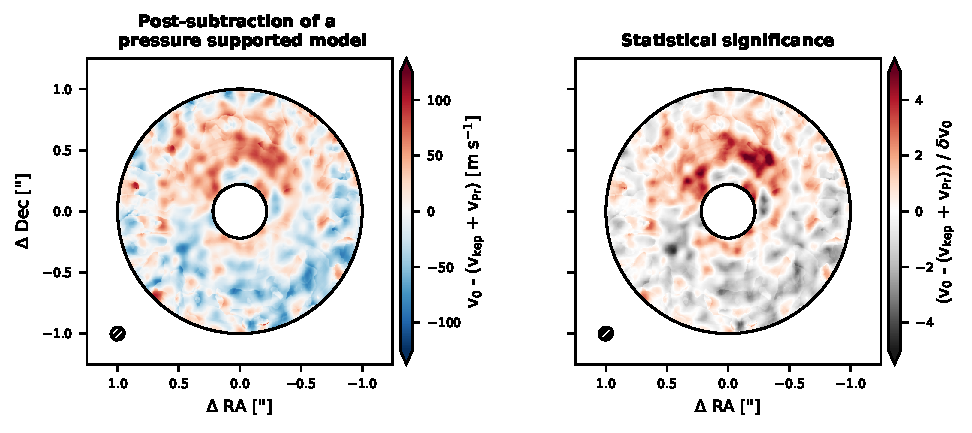
\includegraphics[width = 0.99\textwidth]{figures/garg_arc.pdf}
    \caption{Velocity residuals of the $^{12}$CO observations of HD~169142 calculated by the subtraction of a rotation profile including pressure support (left). Also shown is the residual velocities divided by the uncertainty in the peak velocity (right). The beam size is plotted in the bottom left corner of each panel, while the masked inner and outer regions are filled white \citep{garg2022}.}
    \label{fig:garg_arc}
\end{figure}

\subsection{Semi-Analytical Modelling}

Notably, the feature we detected overlaps with the point source found in \citet{gratton2019} at a PA of $43.8^\circ$ and radial separation of $38$ au.
If the point source is a indeed a planet, perhaps the kinematic arc is associated with the velocity perturbations induced by the tidal forcing of the planet.
To test this scenario, we constructed semi-analytic models of the wake produced by a planet placed in the disk at the location of the \citet{gratton2019} point source using \textsc{wakeflow}.
We chose power law profiles for the unperturbed disk of $c \propto r^{-0.2}$ and $\Sigma \propto r^{-1}$, as well as an aspect ratio of $(H/r)_{\rm p}=0.08$.
The central star mass was chosen as $M_\star = 1.47 \, \mathrm{M_\odot}$ from the best-fitting model described in the previous section.
We used two $M_{\rm p}$ values of $1 \, \mathrm{M_J}$ and $10 \, \mathrm{M_J}$.

After the \textsc{wakeflow} models were calculated, we used the Monte Carlo radiation transfer code \textsc{mcfost} \citep{pinte2006,pinte2009} to generate synthetic $^{12}$CO $J=2-1$ observations.
The total gas mass of the model was set to $10^{-2} \, \mathrm{M_\odot}$ \citep{toci2019} and the gas-to-dust ratio was set to 100.
We use Mie theory \citep{mie1908} to calculate the optical properties of the dust grains, and assume that their size $a$ is distributed as $dn(a) \propto a^{-3.5} da$ where $n(a)$ is the number density of grains with size $a$.
The range of dust grain sizes used was between $0.03 \, \mathrm{\mu m}$ and $1$ mm, and they were taken to have a silicate composition \citep{weingartner2001}.
We assumed equal dust and gas temperatures, as well as local thermodynamic equilibrium.
The central star was modelled as an isotropically radiating blackbody, and $12.8\times 10^6$ packets were used to compute the dust temperature structure.
The relative CO abundance was taken to be $10^{-4}$, and the effects of CO freeze-out at $T < 20\, \mathrm{K}$, and photodissociation and photodesorption in regions of high UV were included following Appendix B of \citet{pinte2018}.
The resultant channel maps had a channel spacing of $32 \, \mathrm{m/s}$, and the synthetic cubes were subsequently convolved spatially with a Gaussian of width $0.1"$ to replicate the beam size in the observations, as well as spectrally with a Hanning function of width $167 \, \mathrm{m/s}$ to replicate the effects of the correlator.

To create sky-plane velocity residuals, the cubes were collapsed spectrally in the same way as for the observations.
This whole process was then repeated except for models were the planet perturbations are absent, and residuals were calculated as the different between the two velocity maps.
These residuals are presented in Figure \ref{fig:garg_analytics}.
Comparing these with Figure \ref{fig:garg_arc}, we see that in neither case do the analytic models recreate the arc found observationally.
The $1 \, \mathrm{M_J}$ planet model contains kinematic deviations that are far smaller than those observed.
On the other hand, the $10 \, \mathrm{M_J}$ produces residuals that while similar in amplitude differ from the observations in shape, location and sign.
Of the two models, the $10 \, \mathrm{M_J}$ is more compatible with the observations, but it still performs poorly.

Since the disk is nearly face-on, the observed kinematic structure may be dominated by vertical motions which are absent in the analytical models.
This may help to explain why the arc was absent in the $^{13}$CO and C$^{18}$O observations, since these trace the disk structure closer to the mid-plane.
For example, buoyancy spirals \citep{zhu2012,bae2021} excited by the planet in a thermally-stratified disk can result in significant vertical motions in the upper layers of the disk.
The planet wake in the mid-plane is expected to be dominated by radial motions \citep{rafikov2002a}, which would be hard to detect given the orientation of the disk.

A significant limitation to the analysis performed here is the accuracy of the \textsc{wakeflow} models nearby the planet.
Given the disk aspect ratio and central star mass, the thermal mass is only $\sim 0.5 \, \mathrm{M_J}$.
Thus the two models we have used here contain planets of masses $2 \, M_{\rm th}$ and $20 \, M_{\rm th}$.
In both of these cases the perturbations calculated close to the planet will be overestimated (\citeauthor{fasanoinprep.}, in prep.).
Unfortunately, in this case that is the region we are specifically interested in, since we are supposing that the kinematic arc contains the planet.
It is therefore only reasonable to interpret these results as upper bounds on the size of the perturbations that may be induced by the planet mass in each model.
We thus conclude that to explain the kinematic excess we have detected in the disk through the perturbations induced by an embedded planet requires a planet of no more than $10 \, \mathrm{M_J}$.
%Planet masses were chosen based off the depth of the gas gap observed at $r=38$ au.
%Equation \ref{eq:kanagawa_gap_depth} relates the gap depth $\Sigma_{\rm p} / \Sigma_0$ to the aspect ratio $(H/r)_{\rm p}$, effective viscosity $\alpha$ and planet mass $M_{\rm p} / M_\star$.
%Taking our measured value of $\Sigma_{\rm p} / \Sigma_0 \approx 0.13$ in combination with  
%$(H/r)_{\rm p}=0.08$, and $\alpha=10^{-3}$ \citep{mulders2012,ansdell2018} gives an approximate planet mass of $\sim$
\begin{figure}
    \centering
    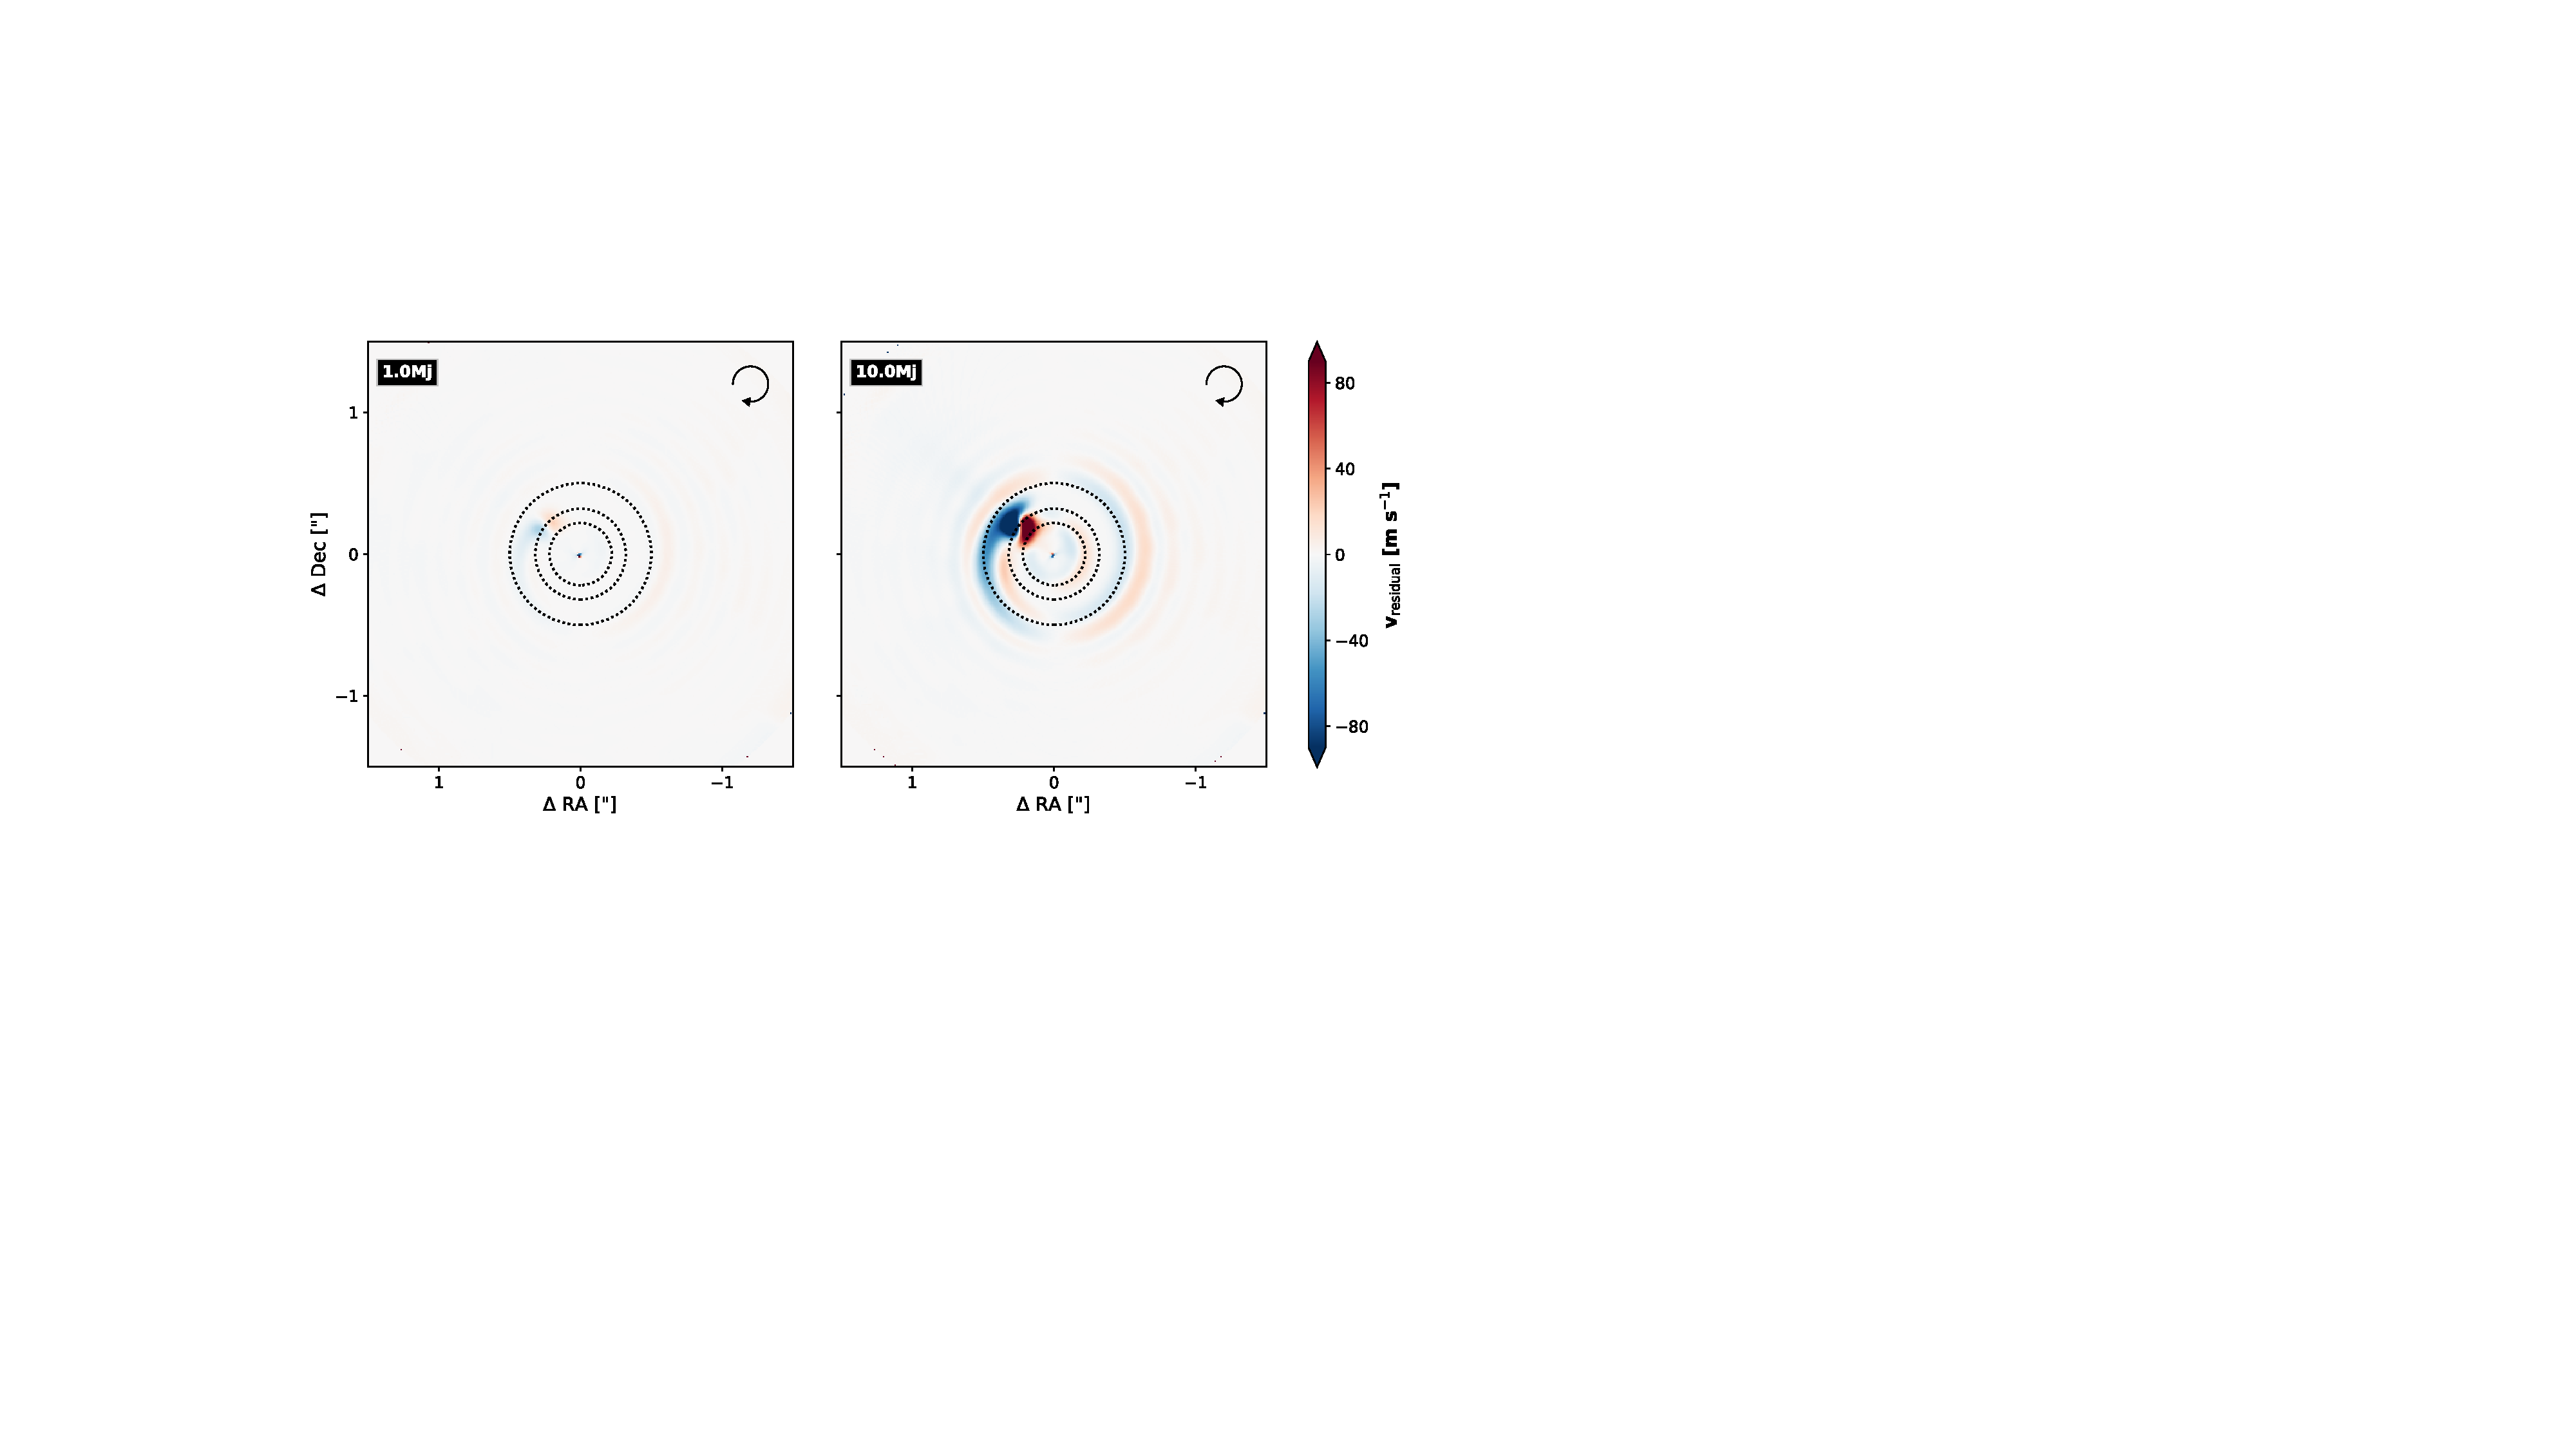
\includegraphics[width = 0.95\textwidth]{figures/garg_analytics_cw.pdf}
    \caption{Velocity perturbations from bulk rotation resulting from the tidal forcing of an embedded planet, calculated using \textsc{wakeflow} and \textsc{mcfost}. The $1 \, \mathrm{M_J}$ planet mass model is shown on the left, while the $10 \, \mathrm{M_J}$ model is shown on the right. The rotation direction of the disk is shown in the top-right of each panel \citep{garg2022}.}
    \label{fig:garg_analytics}
\end{figure}